\documentclass[11pt,a4paper]{article}
\usepackage[T1]{fontenc}
\usepackage[utf8]{inputenc}
\usepackage{lmodern}
\usepackage{textcomp}
\usepackage[left=1.8cm,right=1.8cm,top=3.0cm,bottom=2.2cm,headheight=36pt,headsep=12pt]{geometry}
\usepackage{multicol}
\usepackage{xcolor}
\usepackage{fancyhdr}\usepackage{tikz}
\usepackage{graphicx}
\usepackage{array}
\usepackage{amsmath,amssymb}
\usepackage{setspace}
\usepackage{longtable}
\graphicspath{{../}}
\definecolor{ygreen}{RGB}{46,139,87}\definecolor{dgreen}{RGB}{28,90,56}
\renewcommand{\normalsize}{\fontsize{10.9}{13.4}\selectfont}
\renewcommand{\familydefault}{\rmdefault}
\setlength{\parindent}{0pt}
\setlength{\columnsep}{0.8cm}
\setlength{\columnseprule}{0.4pt}
\setlength{\multicolsep}{3pt plus 1pt minus 1pt}
\renewcommand{\textsubscript}[1]{\ensuremath{_{\text{\fontsize{8}{8}\selectfont #1}}}}
\renewcommand{\textsuperscript}[1]{\ensuremath{^{\text{\fontsize{8}{8}\selectfont #1}}}}
\newcommand{\qn}[1]{\textbf{\fontsize{11.5}{13}\selectfont #1}}
\newcommand{\qsep}{\par\vspace{13pt}}
\newcommand{\fwrule}{\par\vspace{5pt}\noindent\rule{\linewidth}{1.4pt}\par\vspace{7pt}}
\newsavebox{\fitb}
\newcommand{\fitbox}[1]{\sbox{\fitb}{#1}\ifdim\wd\fitb>\linewidth\resizebox{\linewidth}{!}{\usebox{\fitb}}\else\usebox{\fitb}\fi}
\newcommand{\diqqat}[1]{\par\smallskip\noindent\textbf{Diqqat!} #1\par\medskip}
\newcommand{\javob}{\par\nopagebreak[4]\smallskip\noindent\textbf{Javob:} \rule[-2pt]{7.5cm}{0.4pt}\par\smallskip\noindent\textbf{Diqqat!} Javobingizni javoblar varaqasiga ko`chirib yozing.\par\medskip}
\pagestyle{fancy}
\fancyhf{}
\renewcommand{\headrulewidth}{1.6pt}\renewcommand{\headrule}{{\color{ygreen}\hrule height 1.6pt width\headwidth}}
\newcommand{\hdrlogo}{
\begin{tikzpicture}[baseline=0pt]\fill[ygreen,rounded corners=3pt] (0,0) rectangle (0.95,0.95);\node[white,font=\fontsize{24}{26}\bfseries\selectfont] at (0.475,0.47){K};\node[anchor=west,font=\fontsize{16}{18}\bfseries\selectfont,text=dgreen] at (1.15,0.66){KIMYO};\node[anchor=west,font=\footnotesize\scshape,text=gray] at (1.15,0.2){Milliy sertifikat\ \ 2026};\end{tikzpicture}}
\newcommand{\hdrpill}[1]{\begin{tikzpicture}[baseline=0pt]\node[fill=ygreen,text=white,rounded corners=8pt,inner xsep=10pt,inner ysep=5pt,font=\fontsize{13}{15}\bfseries\selectfont] at (0,0.475){#1};\end{tikzpicture}}
\fancyhead[L]{\hdrlogo}
\fancyhead[R]{\hdrpill{12-variant}}

\fancyfoot[C]{\thepage}
\fancypagestyle{first}{\fancyhf{}\renewcommand{\headrulewidth}{1.6pt}\renewcommand{\headrule}{{\color{ygreen}\hrule height 1.6pt width\headwidth}}\fancyhead[L]{\hdrlogo}\fancyhead[R]{\hdrpill{12-variant}}\fancyfoot[C]{\thepage}}
\begin{document}
\normalsize
\thispagestyle{first}
\noindent\textit{Davriy jadvaldan foydalanish mumkin.}
\par\smallskip
\begin{multicols}{2}
\noindent\qn{1.} Qaysi juftliklarda reaksiya boradi? 1) Pb va ZnCl\textsubscript{2}; 2) Al va CuSO\textsubscript{4}; 3) Zn va CuSO\textsubscript{4}; 4) Ag va CuSO\textsubscript{4}

\noindent A)~\textsl{1, 2} \hfill B)~\textsl{2, 3} \hfill C)~\textsl{4} \hfill D)~\textsl{1, 2, 4}\par
\qsep
\noindent\qn{2.} Jadvalda bog`lar hosil qiluvchi atomlarning elektrmanfiyliklari berilgan:
\begin{center}
\renewcommand{\arraystretch}{1.15}
\fitbox{\begin{tabular}{|c|c|c|}\hline
\textbf{Bog`} & \textbf{EM (1-atom)} & \textbf{EM (2-atom)} \\ \hline
H--Cl & 2,1 & 3 \\ \hline
H--O & 2,1 & 3,5 \\ \hline
H--F & 2,1 & 4 \\ \hline
C--O & 2,5 & 3,5 \\ \hline
\end{tabular}}
\end{center}
Qaysi bog` eng qutbli (eng ko`p ionli xarakterga ega)?

\noindent A)~\textsl{H--F} \hfill B)~\textsl{H--Cl} \hfill C)~\textsl{H--O} \hfill D)~\textsl{C--O}\par
\qsep
\noindent\qn{3.} Rasmda neytral atom elektron qavatlarining orbital diagrammasi (kataklar -- orbitallar, o`qlar -- elektronlar) berilgan.
\begin{center}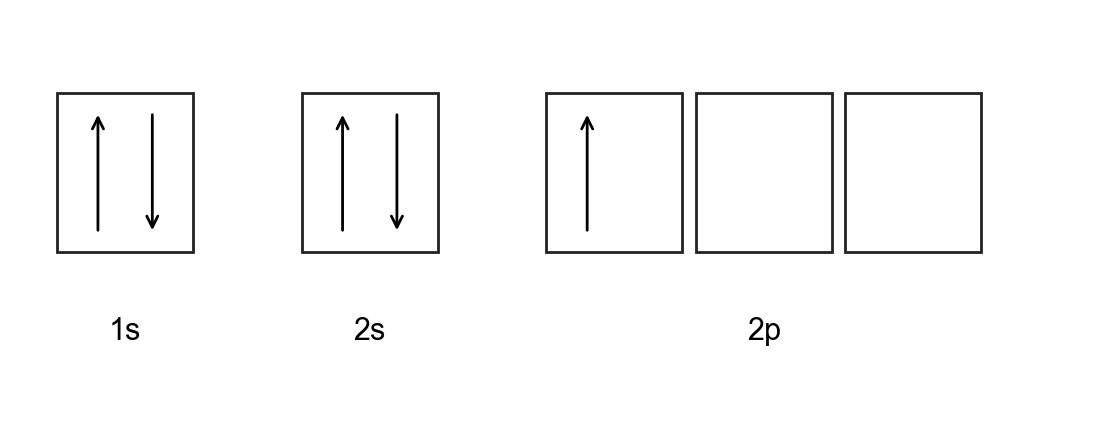
\includegraphics[width=0.86\linewidth]{rasmlar/gen/or_588848.png}\end{center}
Diagramma qaysi element atomiga tegishli?

\noindent A)~\textsl{kislorod} \hfill B)~\textsl{azot} \hfill C)~\textsl{bor} \hfill D)~\textsl{uglerod}\par
\qsep
\noindent\qn{4.} 34-tartib raqamli element atomida n = 3 va l = 2 bo`lgan elektronlar \textbf{sonini aniqlang.}

\noindent A)~\textsl{10} \hfill B)~\textsl{11} \hfill C)~\textsl{9} \hfill D)~\textsl{12}\par
\qsep
\noindent\qn{5.} Massa soni 238, zaryadi 92 bo`lgan yadro massa soni 206, zaryadi 82 bo`lgan yadroga aylandi ($\alpha$ va $\beta$\textsuperscript{$-$} parchalanish). Nechta $\beta$\textsuperscript{$-$}-zarra chiqarilgan?

\noindent A)~\textsl{7} \hfill B)~\textsl{5} \hfill C)~\textsl{8} \hfill D)~\textsl{6}\par
\qsep
\noindent\qn{6.} O\textsubscript{2} va CO\textsubscript{2} gazlari 1 : 3 hajmiy nisbatda aralashtirildi. Aralashmaning vodorodga nisbatan \textbf{zichligini aniqlang.}

\noindent A)~\textsl{41} \hfill B)~\textsl{21,5} \hfill C)~\textsl{19} \hfill D)~\textsl{20,5}\par
\qsep
\noindent\qn{7.} Konsentratsiyasi bir xil (0,1 mol/l) eritmalarning pH qiymatlari diagrammada berilgan.
\begin{center}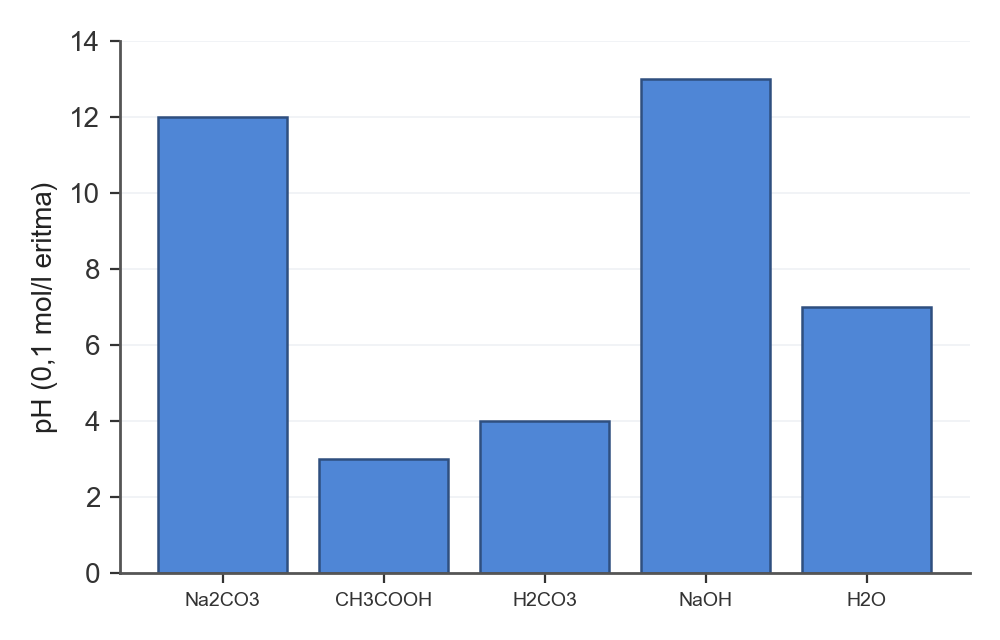
\includegraphics[width=0.86\linewidth]{rasmlar/gen/pb_v12_0.png}\end{center}
Na\textsubscript{2}CO\textsubscript{3} eritmasining pH i neytraldan necha birlikka farq qiladi?

\noindent A)~\textsl{5} \hfill B)~\textsl{6} \hfill C)~\textsl{1000000} \hfill D)~\textsl{50}\par
\qsep
\noindent\qn{8.} Mg va Al aralashmasi tarkibida aralashmadagi atomlarning umumiy soni 0,6$\cdot$N\textsubscript{A}. Aralashmaning massasi 15,9 g. Aralashmadagi Mg ning \textbf{massasini (g) toping.}

\noindent A)~\textsl{13,5} \hfill B)~\textsl{2,4} \hfill C)~\textsl{4,8} \hfill D)~\textsl{7,95}\par
\qsep
\noindent\qn{9.} Fe plastinka 16 g CuSO\textsubscript{4} ni tutgan eritmaga tushirildi va Cu to`liq ajralib chiqquncha ushlab turildi. Plastinka massasi necha gramm ortadi?

\noindent A)~\textsl{1,6} \hfill B)~\textsl{0,8} \hfill C)~\textsl{0,4} \hfill D)~\textsl{16}\par
\qsep
\noindent\qn{10.} Faqat qaytaruvchi bo`la oladigan \textbf{ionlarni aniqlang}: 1) Fe\textsuperscript{3+}; 2) I\textsuperscript{$-$}; 3) K\textsuperscript{+}; 4) Mn\textsuperscript{7+} (MnO\textsubscript{4}\textsuperscript{$-$})

\noindent A)~\textsl{2} \hfill B)~\textsl{3} \hfill C)~\textsl{1, 4} \hfill D)~\textsl{2, 4}\par
\qsep
\noindent\qn{11.} Laboratoriyada NaNO\textsubscript{3} eritmalari quyidagicha tayyorlangan:
\begin{center}
\renewcommand{\arraystretch}{1.15}
\fitbox{\begin{tabular}{|c|c|c|}\hline
\textbf{Idish} & \textbf{Eritma massasi, g} & \textbf{$\omega$(NaNO\textsubscript{3}), \%} \\ \hline
A & 150 & 20 \\ \hline
B & 100 & 35 \\ \hline
\end{tabular}}
\end{center}
Bu ikki eritma bir idishga quyilib, yangi eritmadagi NaNO\textsubscript{3} ning massa ulushi (\%) qancha bo`ladi?

\noindent A)~\textsl{27,5} \hfill B)~\textsl{55} \hfill C)~\textsl{26} \hfill D)~\textsl{29}\par
\qsep
\noindent\qn{12.} 20 l H\textsubscript{2} va 15 l O\textsubscript{2} aralashmasi reaksiyaga kirishdi. Reaksiyadan keyingi gaz aralashmasining \textbf{hajmini (l) aniqlang.}

\noindent A)~\textsl{35} \hfill B)~\textsl{20} \hfill C)~\textsl{25} \hfill D)~\textsl{5}\par
\qsep
\noindent\qn{13.} Quyidagi jadvalda K\textsubscript{2}SO\textsubscript{4} tuzining eritmalari keltirilgan:
\begin{center}
\renewcommand{\arraystretch}{1.15}
\fitbox{\begin{tabular}{|c|c|c|}\hline
\textbf{No.} & \textbf{m(eritma), g} & \textbf{$\omega$, \%} \\ \hline
I & 200 & 20 \\ \hline
II & 200 & 40 \\ \hline
\end{tabular}}
\end{center}
Eritmalar aralashtirilib, ustiga 100 g suv qo`shildi. Oxirgi eritmadagi tuzning massa \textbf{ulushini (\%) toping.}

\noindent A)~\textsl{30} \hfill B)~\textsl{60} \hfill C)~\textsl{21,6} \hfill D)~\textsl{24}\par
\qsep
\noindent\qn{14.} Qaysi juftliklar o`zaro reaksiyaga kirishadi? 1) Fe va HCl; 2) Fe\textsubscript{2}O\textsubscript{3} va H\textsubscript{2}O; 3) CuSO\textsubscript{4} va NaOH; 4) CuO va H\textsubscript{2}

\noindent A)~\textsl{1, 2, 4} \hfill B)~\textsl{2, 3} \hfill C)~\textsl{1, 3, 4} \hfill D)~\textsl{1, 3}\par
\qsep
\noindent\qn{15.} Cu(NO\textsubscript{3})\textsubscript{2} qizdirilganda qanday moddalar hosil bo`ladi?

\noindent\begin{tabular}{@{}p{0.47\linewidth}@{}p{0.47\linewidth}@{}}
A)~\textsl{ZnO, NO\textsubscript{2} va O\textsubscript{2}} & B)~\textsl{CuO, NO\textsubscript{2} va O\textsubscript{2}} \\
C)~\textsl{Ag, NO\textsubscript{2} va O\textsubscript{2}} & D)~\textsl{NaNO\textsubscript{2} va O\textsubscript{2}} \\
\end{tabular}\par
\qsep
\noindent\qn{16.} Probirkalardagi eritmalar: NaCl, Na\textsubscript{2}CO\textsubscript{3}, Na\textsubscript{2}SO\textsubscript{4} ni alohida probirkalarda ajratish uchun qaysi reagent(lar) yetarli? 1) lakmus; 2) HCl; 3) BaCl\textsubscript{2} va lakmus; 4) BaCl\textsubscript{2}

\noindent A)~\textsl{1, 3} \hfill B)~\textsl{1} \hfill C)~\textsl{3} \hfill D)~\textsl{2, 3}\par
\qsep
\noindent\qn{17.} Quyidagi jarayonlar qanday kuzatuvlar bilan boradi? To`g`ri ta'riflangan \textbf{jarayonlarni belgilang.} 1) AlCl\textsubscript{3} eritmasiga avval oz, so`ng mo`l NaOH eritmasi qo`shilganda: oq cho`kma tushadi, keyin cho`kma erib ketadi; 2) FeCl\textsubscript{3} eritmasiga avval NaOH, so`ng mo`l HCl eritmasi qo`shilganda: qo`ng`ir-qizil cho`kma tushadi, keyin cho`kma erib, sariq eritma hosil bo`ladi; 3) NaOH eritmasiga CuSO\textsubscript{4} eritmasi tomchilab qo`shilganda (ishqor mo`l): ko`k cho`kma tushadi, keyin cho`kma erib to`q ko`k eritma hosil bo`ladi; 4) ZnSO\textsubscript{4} eritmasiga avval oz, so`ng mo`l NaOH eritmasi qo`shilganda: oq cho`kma tushadi, keyin cho`kma erimasdan qoladi

\noindent A)~\textsl{1, 3} \hfill B)~\textsl{1, 2} \hfill C)~\textsl{4} \hfill D)~\textsl{2, 3}\par
\qsep
\noindent\qn{18.} 0,2 mol NaOH tutgan eritmadan 0,15 mol CO\textsubscript{2} o`tkazildi. Hosil bo`lgan NaHCO\textsubscript{3} \textbf{massasini (g) aniqlang.}

\noindent A)~\textsl{8,4} \hfill B)~\textsl{2,1} \hfill C)~\textsl{8} \hfill D)~\textsl{4,2}\par
\qsep
\noindent\qn{19.} CuSO\textsubscript{4} tuzining kristallogidratida suvning massa ulushi 36\% ni tashkil etadi. Kristallogidrat formulasidagi suv molekulalari \textbf{sonini (n) toping.}

\noindent A)~\textsl{8} \hfill B)~\textsl{10} \hfill C)~\textsl{4} \hfill D)~\textsl{5}\par
\qsep
\noindent\qn{20.} Probirkalardagi organik moddalar: etanol, etanal, glitserin ni alohida probirkalarda ajratish uchun qaysi reagent(lar) yetarli? 1) Cu(OH)\textsubscript{2} (qizdirilganda) va [Ag(NH\textsubscript{3})\textsubscript{2}]OH; 2) [Ag(NH\textsubscript{3})\textsubscript{2}]OH va FeCl\textsubscript{3}; 3) Cu(OH)\textsubscript{2} (qizdirilganda); 4) [Ag(NH\textsubscript{3})\textsubscript{2}]OH va Na metali

\noindent A)~\textsl{1, 2, 3} \hfill B)~\textsl{4} \hfill C)~\textsl{1, 3} \hfill D)~\textsl{1, 2}\par
\qsep
\noindent\qn{21.} Aldegid va ketonlar haqida qaysi fikrlar to`g`ri? 1) Formalin --- formaldegidning 40\% li eritmasi; 2) Aldegidlar "kumush ko`zgu" reaksiyasini beradi; 3) Formaldegid gaz holatda, suvda yaxshi eriydi; 4) Ketonlar kuchsiz oksidlovchilar bilan oksidlanmaydi

\noindent\begin{tabular}{@{}p{0.47\linewidth}@{}p{0.47\linewidth}@{}}
A)~\textsl{1, 3, 4} & B)~\textsl{1, 2, 4} \\
C)~\textsl{1, 2, 3, 4} & D)~\textsl{2, 3, 4} \\
\end{tabular}\par
\qsep
\noindent\qn{22.} Murakkab efirlar va yog`lar haqida qaysi fikrlar to`g`ri? 1) Dietil efir spirtdan yuqori haroratda qaynaydi; 2) Etilatsetat efir hidli suyuqlik; 3) Efirlanish reaksiyasi qaytmas; 4) Murakkab efirlarning gidrolizi ishqoriy muhitda qaytmas

\noindent A)~\textsl{1, 4} \hfill B)~\textsl{2, 4} \hfill C)~\textsl{2, 3, 4} \hfill D)~\textsl{3}\par
\qsep
\noindent\qn{23.} Benzol va toluol aralashmasi yondirilganda 2,7 mol CO\textsubscript{2} va 1,5 mol suv hosil bo`ldi. Aralashmadagi benzolning mol \textbf{ulushini (\%) aniqlang.}

\noindent A)~\textsl{25} \hfill B)~\textsl{75} \hfill C)~\textsl{22} \hfill D)~\textsl{50}\par
\qsep
\noindent\qn{24.} 486 g kraxmal gidrolizlanib (unum 80\%) glukoza olindi, glukoza esa spirtli bijg`ishga uchradi (unum 90\%). Barcha reaksiyalar 2 atm bosimda olib borildi. Hosil bo`lgan etanol \textbf{massasini (g) toping.}

\noindent A)~\textsl{99,4} \hfill B)~\textsl{397,4} \hfill C)~\textsl{220,8} \hfill D)~\textsl{198,7}\par
\qsep
\noindent\qn{25.} 81 g (C\textsubscript{6}H\textsubscript{10}O\textsubscript{5})n dan quyidagi sxema bo`yicha divinil kauchuk olindi: (C\textsubscript{6}H\textsubscript{10}O\textsubscript{5})n $\to$ C\textsubscript{6}H\textsubscript{12}O\textsubscript{6} $\to$ C\textsubscript{2}H\textsubscript{5}OH $\to$ CH\textsubscript{2}=CH--CH=CH\textsubscript{2} $\to$ (--CH\textsubscript{2}--CH=CH--CH\textsubscript{2}--)n. Bosqichlarning unumi ketma-ket 60\%, 40\%, 50\%, 75\% ni tashkil qiladi. Olingan divinil kauchuk \textbf{massasini (g) aniqlang.}

\noindent A)~\textsl{2,43} \hfill B)~\textsl{4,86} \hfill C)~\textsl{1,21} \hfill D)~\textsl{3,24}\par
\qsep
\noindent\qn{26.} 11,2 l (n.sh.) CH\textsubscript{4} dan quyidagi sxema bo`yicha kumush olindi: CH\textsubscript{4} $\to$ C\textsubscript{2}H\textsubscript{2} $\to$ CH\textsubscript{3}CHO $\to$ Ag. Bosqichlarning unumi ketma-ket 80\%, 90\%, 50\% ni tashkil qiladi. Olingan kumush \textbf{massasini (g) aniqlang.}

\noindent A)~\textsl{38,88} \hfill B)~\textsl{9,72} \hfill C)~\textsl{27} \hfill D)~\textsl{19,44}\par
\qsep
\noindent\qn{27.} Chumoli va akril kislota aralashmasi mo`l NaHCO\textsubscript{3} eritmasi bilan ta'sirlashganda 6,72 l (n.sh.) gaz ajraldi. Shu miqdordagi aralashma ammiakli kumush oksid bilan qizdirilganda 43,2 g kumush hosil bo`ldi. Qizdirish 30 daqiqa davom etdi. Aralashmadagi akril kislotaning \textbf{massasini (g) toping.}

\noindent A)~\textsl{9,2} \hfill B)~\textsl{14,4} \hfill C)~\textsl{3,6} \hfill D)~\textsl{7,2}\par
\qsep
\noindent\qn{28.} 61,5 g C\textsubscript{6}H\textsubscript{5}NO\textsubscript{2} dan quyidagi sxema bo`yicha fenilammoniy xlorid olindi: C\textsubscript{6}H\textsubscript{5}NO\textsubscript{2} $\to$ C\textsubscript{6}H\textsubscript{5}NH\textsubscript{2} $\to$ [C\textsubscript{6}H\textsubscript{5}NH\textsubscript{3}]Cl. Bosqichlarning unumi ketma-ket 90\%, 40\% ni tashkil qiladi. Olingan fenilammoniy xlorid \textbf{massasini (g) aniqlang.}

\noindent A)~\textsl{23,31} \hfill B)~\textsl{46,62} \hfill C)~\textsl{11,66} \hfill D)~\textsl{58,28}\par
\qsep
\noindent\qn{29.} 92 g C\textsubscript{2}H\textsubscript{5}OH dan quyidagi sxema bo`yicha 16,2 g divinil kauchuk olindi: 2C\textsubscript{2}H\textsubscript{5}OH $\to$ CH\textsubscript{2}=CH--CH=CH\textsubscript{2} $\to$ (--CH\textsubscript{2}--CH=CH--CH\textsubscript{2}--)n. Dastlabki 1 bosqichning unumi ketma-ket 75\% ga teng. Oxirgi bosqichning \textbf{unumini (\%) aniqlang.}

\noindent A)~\textsl{20} \hfill B)~\textsl{40} \hfill C)~\textsl{60} \hfill D)~\textsl{32}\par
\qsep
\noindent\qn{30.} Raqamlangan (1--4) probirkalarda HCl, Na\textsubscript{2}S, NaOH, Pb(NO\textsubscript{3})\textsubscript{2} eritmalari tartibsiz holda berilgan. Quyidagi kuzatuvlar asosida moddalarni probirka raqami bilan moslang. 2- va 3-probirkalardagi eritmalar aralashtirilganda bir-birini neytrallaydi. 1- va 4-probirkalardagi eritmalar aralashtirilganda qora cho`kma tushadi. 1- va 2-probirkalardagi eritmalar aralashtirilganda chirigan tuxum hidli gaz ajraladi.
\noindent A)~\textsl{1-Na\textsubscript{2}S, 2-HCl, 3-NaOH, 4-Pb(NO\textsubscript{3})\textsubscript{2}}\par
\noindent B)~\textsl{1-NaOH, 2-HCl, 3-Na\textsubscript{2}S, 4-Pb(NO\textsubscript{3})\textsubscript{2}}\par
\noindent C)~\textsl{1-Na\textsubscript{2}S, 2-NaOH, 3-HCl, 4-Pb(NO\textsubscript{3})\textsubscript{2}}\par
\noindent D)~\textsl{1-HCl, 2-Na\textsubscript{2}S, 3-NaOH, 4-Pb(NO\textsubscript{3})\textsubscript{2}}\par
\qsep
\noindent\qn{31.} Quyidagi aralashmalarni ajratish usullarini mos qatorda \textbf{ko`rsating.} Aralashmalar: 1) yod va osh tuzi; 2) dengiz suvidan toza suv olish; 3) temir va mis kukunlari. Usullar: a) magnit yordamida; b) distillash (haydash); c) sublimatsiya (qizdirib, bug`ini sovitish); d) tindirish va filtrlash.

\noindent\begin{tabular}{@{}p{0.47\linewidth}@{}p{0.47\linewidth}@{}}
A)~\textsl{1-b, 2-a, 3-d} & B)~\textsl{1-a, 2-d, 3-b} \\
C)~\textsl{1-c, 2-b, 3-a} & D)~\textsl{1-c, 2-a, 3-b} \\
\end{tabular}\par
\qsep
\noindent\qn{32.} Rasmdagi tajribada loyqa suv filtrdan o`tkazilganda qaysi modda filtr qog`ozida qoladi?
\begin{center}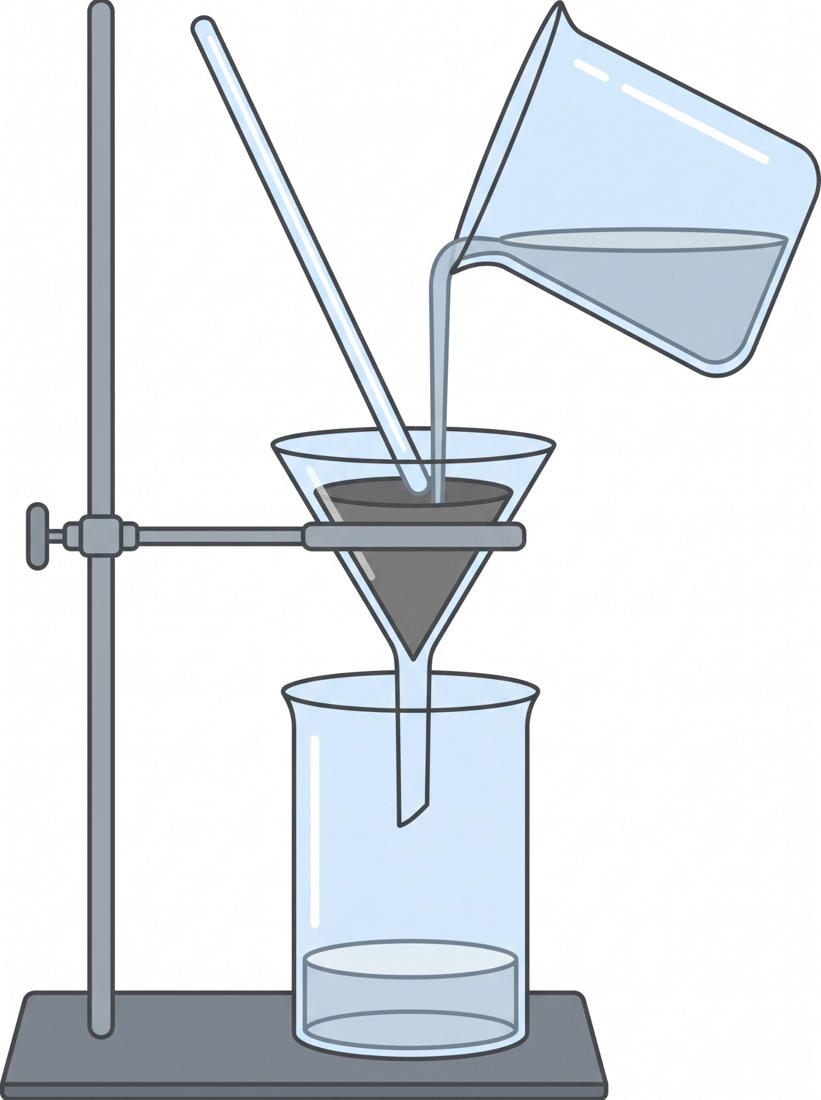
\includegraphics[width=0.86\linewidth]{rasmlar/darslik/d_filtr.png}\end{center}
\noindent A)~\textsl{suv molekulalari}\par
\noindent B)~\textsl{suvda erimaydigan qattiq zarrachalar}\par
\noindent C)~\textsl{etanol}\par
\noindent D)~\textsl{suvda erigan osh tuzi   ---}\par
\qsep
\end{multicols}
\medskip
\noindent\setlength{\fboxsep}{0pt}\fbox{\begin{tabular}{p{0.74\linewidth}|p{0.2\linewidth}}
\parbox[t]{0.72\linewidth}{\vspace{3pt}\textbf{Topshiriqlar (33--35) va javob variant (A--F)larini o`zaro to`g`ri moslashtiring.} 75,2 g Cu(NO\textsubscript{3})\textsubscript{2} doimiy massagacha qizdirildi, ajralgan gazlar aralashmasi 100 g suvga yuborildi.
\vspace{3pt}} & \parbox[t]{0.19\linewidth}{\vspace{3pt}A~\textsl{32}\\[3pt]
B~\textsl{50,4}\\[3pt]
C~\textsl{75,6}\\[3pt]
D~\textsl{35,2}\\[3pt]
E~\textsl{25,2}\\[3pt]
F~\textsl{40,32}}\\ \hline
\parbox[t]{0.72\linewidth}{\vspace{2pt}\textbf{33. Qattiq qoldiq massasini (g) aniqlang.}\vspace{2pt}} & \\ \hline
\parbox[t]{0.72\linewidth}{\vspace{2pt}\textbf{34. Hosil bo`lgan nitrat kislota massasini (g) toping.}\vspace{2pt}} & \\ \hline
\parbox[t]{0.72\linewidth}{\vspace{2pt}\textbf{35. Olingan eritmada nitrat kislotaning massa ulushini (\%) hisoblang.}\vspace{2pt}} & 
\end{tabular}}
\par\bigskip
\noindent\qn{36.} 15\% li va 30\% li tuz eritmalari massalar nisbati 3 : 2 bo`lgan holda aralashtirildi. Tajriba 10 daqiqa davom etdi. Hosil bo`lgan eritmaning massa \textbf{ulushini (\%) hisoblang.}
\javob\qsep
\noindent\qn{37.} Ketma-ket ulangan ikkita elektrolizyordan (CuSO\textsubscript{4} va AgNO\textsubscript{3} eritmalari, inert elektrodlar) tok o`tkazildi. Birinchi elektrolizyor katodida 6,4 g mis ajraldi. Elektrolizyorning hajmi 3 l. Ikkala elektrolizyor anodlarida ajralgan kislorodning umumiy \textbf{hajmini (l, n.sh.) toping} (anodda ikkalasida ham O\textsubscript{2} ajraladi).
\javob\qsep
\noindent\qn{38.} Alyuminiy (0,2 mol) va magniy (0,2 mol) aralashmasi mo`l xlorid kislotada eritildi. Reagent (xlorid kislota) eritmasining massa ulushi 36\% va zichligi 1,4 g/ml; u mo`l miqdorda olingan. Ajralgan vodorodning \textbf{hajmini (l, n.sh.) aniqlang.}
\javob\qsep
\noindent\qn{39.} Bir asosli to`yingan karbon kislotaning 52,8 g miqdori mo`l NaHCO\textsubscript{3} bilan ta'sirlashganda 13,44 l (n.sh.) gaz ajraldi. Shu kislotaning 1/3 qismi mo`l etanol bilan esterlandi (efir unumi 3/4). Barcha reaksiyalar 1,5 atm bosimda olib borildi. Hosil bo`lgan murakkab efirning \textbf{massasini (g) toping.}
\javob\qsep
\noindent\qn{40.} Bir atomli to`yingan noma'lum spirtning 29,6 g miqdori natriy bilan ta'sirlashganda 4,48 l (n.sh.) vodorod ajraldi. Shu spirtning 3/4 qismi mis(II) oksid bilan oksidlandi, hosil bo`lgan modda mo`l ammiakli kumush oksid eritmasi bilan qizdirildi. Qizdirish 20 daqiqa davom etdi. Ajralgan kumush \textbf{massasini (g) toping.}
\javob\qsep
\par\bigskip\begin{center}\textbf{\fontsize{13}{15}\selectfont YOZMA ISH}\end{center}
\noindent\qn{41.} \textbf{Topshiriqni bajarish jarayonida barcha reaksiya tenglamalarini yozing. Miqdoriy va arifmetik hisoblashlarni (unga asos bo`lgan usul yoki formulani ko`rsatgan holda) uzviy ketma-ketlikda bajaring.}\par\smallskip
Tarkibi XSO\textsubscript{4}$\cdot$nH2O bo`lgan (\textit{X} -- oksidlanish darajasi +2 bo`lgan metall) kristallogidratning 26,3 g namunasida suvning massa ulushi 41,1\% ni tashkil etadi. Namuna suvda eritilib, mo`l BaCl\textsubscript{2} eritmasi qo`shilganda 23,3 g cho`kma tushdi. Cho`kma ajratilgach, filtratga mo`l NaOH eritmasi qo`shilib, hosil bo`lgan gidroksid doimiy massagacha kuydirildi.\par
\noindent 1)\ Barcha reaksiyalarning tenglamalarini yozing; kristallogidratning molyar massasini va tuzdagi (suvsiz) qismining molyar massasini hisoblang.\par
\noindent 2)\ \textit{X} metallni aniqlang va n ning qiymatini toping.\par
\noindent 3)\ Namunadagi XSO\textsubscript{4} ning (suvsiz) massasini va kristallizatsion suv massasini (g) hisoblang.\par
\noindent 4)\ Filtratga sarflangan NaOH ning minimal miqdorini (mol) toping.\par
\noindent 5)\ Kuydirishdan hosil bo`lgan oksid massasini (g) aniqlang va u namuna massasining necha foizini tashkil etishini toping.\par
\diqqat{Mazkur topshiriq kengaytirilgan javobni talab etib, uning yechilish usuli va shu usul asosidagi barcha hisoblash amallari javoblar varaqasida aks etishi lozim.}\qsep
\noindent\qn{42.} Organik moddalarning xossalarini bilgan holda reaksiya tenglamalarini tugallang va tenglashtiring. 3- va 5-reaksiyalarda hosil bo`lgan asosiy organik mahsulotlarni sistematik nomenklatura bo`yicha nomlang. Hosil bo`lgan organik moddalarning tuzilish formulalarini yozing.\par
\noindent 1)\ H\textsubscript{2}N--CH\textsubscript{2}--COOH + HCl $\to$\par
\noindent 2)\ CH\textsubscript{3}--CH\textsubscript{2}--OH + CH\textsubscript{3}--COOH (H\textsubscript{2}SO\textsubscript{4}, t) $\rightleftarrows$\par
\noindent 3)\ H\textsubscript{2}N--CH\textsubscript{2}--COOH + NaOH $\to$\par
\noindent 4)\ CH\textsubscript{3}--CH\textsubscript{2}--CHO + Ag\textsubscript{2}O (NH\textsubscript{3}, t) $\to$\par
\noindent 5)\ C\textsubscript{6}H\textsubscript{5}--CH\textsubscript{3} + KMnO\textsubscript{4} + H\textsubscript{2}SO\textsubscript{4} (t) $\to$\par
\noindent 6)\ H\textsubscript{2}N--CH\textsubscript{2}--COOH + H\textsubscript{2}N--CH\textsubscript{2}--COOH $\to$\par
\noindent 7)\ CH$\equiv$CH + H\textsubscript{2}O (Hg\textsuperscript{2+}, H\textsuperscript{+}) $\to$\par
\diqqat{Mazkur topshiriq kengaytirilgan javobni talab etib, uning yechilish usuli va shu usul asosidagi barcha hisoblash amallari javoblar varaqasida aks etishi lozim.}\qsep
\noindent\qn{43.} \textbf{Topshiriqni bajarish jarayonida barcha reaksiya tenglamalarini yozing. Miqdoriy va arifmetik hisoblashlarni (unga asos bo`lgan usul yoki formulani ko`rsatgan holda) uzviy ketma-ketlikda bajaring.}\par\smallskip
Alyuminiy va noma'lum \textit{X} metalldan (\textit{X} -- oksidlanish darajasi +2 bo`lgan metall) iborat 8,3 g aralashma mo`l NaOH eritmasi bilan ta'sirlashganda 3,36 l (n.sh.) gaz ajraldi. Shunday massali ikkinchi namuna mo`l xlorid kislotada eritilganda 5,6 l (n.sh.) gaz ajraldi. Xlorid kislotali eritmaga mo`l NaOH eritmasi qo`shilib, cho`kma ajratildi, havoda to`liq oksidlanguncha tutildi va kuydirildi; filtratdan mo`l CO\textsubscript{2} o`tkazildi. Reagent (NaOH) eritmasining massa ulushi 36\% va zichligi 1,4 g/ml; u mo`l miqdorda olingan. Hosil bo`lgan Al(OH)\textsubscript{3} nitrat kislotada eritildi, eritma bug`latilib, qoldiq doimiy massagacha qizdirildi, ajralgan gazlar suvga yuttirildi.\par
\noindent 1)\ Barcha reaksiyalarning tenglamalarini yozing va tenglashtiring.\par
\noindent 2)\ Aralashmadagi Al va \textit{X} ning miqdorlarini (mol) aniqlang va \textit{X} metallni toping.\par
\noindent 3)\ Aralashmadagi metallarning massa ulushlarini (\%) hisoblang. Al(OH)\textsubscript{3} ni eritish uchun sarflangan HNO\textsubscript{3} miqdorini (mol) toping.\par
\noindent 4)\ Kuydirishdan hosil bo`lgan qattiq moddaning formulasini aniqlang va massasini (g) hisoblang. Al(NO\textsubscript{3})\textsubscript{3} qizdirilganda ajralgan gazlar hajmini (l, n.sh.) hisoblang.\par
\noindent 5)\ Filtratdan CO\textsubscript{2} o`tkazilganda hosil bo`lgan cho`kma massasini (g) toping. Gazlar suvga yuttirilganda hosil bo`lgan HNO\textsubscript{3} massasini (g) aniqlang.\par
\diqqat{Mazkur topshiriq kengaytirilgan javobni talab etib, uning yechilish usuli va shu usul asosidagi barcha hisoblash amallari javoblar varaqasida aks etishi lozim.}\qsep
\newpage
\noindent\textbf{\fontsize{13}{15}\selectfont 12-variant}\hfill \textbf{Javoblar kaliti}\par\smallskip\hrule\smallskip
\textit{Faqat o`qituvchi uchun.}\par\medskip
\noindent\textbf{1--32-savollar}\par\smallskip
\noindent\begin{tabular}{|c|c|c|c|c|c|c|c|c|c|c|c|c|c|c|c|}\hline
\textbf{1} & \textbf{2} & \textbf{3} & \textbf{4} & \textbf{5} & \textbf{6} & \textbf{7} & \textbf{8} & \textbf{9} & \textbf{10} & \textbf{11} & \textbf{12} & \textbf{13} & \textbf{14} & \textbf{15} & \textbf{16}\\\hline
\textsl{B} & \textsl{A} & \textsl{C} & \textsl{A} & \textsl{D} & \textsl{D} & \textsl{A} & \textsl{B} & \textsl{B} & \textsl{A} & \textsl{C} & \textsl{C} & \textsl{D} & \textsl{C} & \textsl{B} & \textsl{C}\\\hline
\textbf{17} & \textbf{18} & \textbf{19} & \textbf{20} & \textbf{21} & \textbf{22} & \textbf{23} & \textbf{24} & \textbf{25} & \textbf{26} & \textbf{27} & \textbf{28} & \textbf{29} & \textbf{30} & \textbf{31} & \textbf{32}\\\hline
\textsl{B} & \textsl{D} & \textsl{D} & \textsl{C} & \textsl{C} & \textsl{B} & \textsl{A} & \textsl{D} & \textsl{A} & \textsl{D} & \textsl{D} & \textsl{A} & \textsl{B} & \textsl{A} & \textsl{C} & \textsl{B}\\\hline
\end{tabular}\par\medskip
\noindent\textbf{33--35-savollar}\par\smallskip
\noindent\begin{tabular}{|c|c|c|}\hline \textbf{No} & \textbf{Javob} & \textbf{Qiymat}\\\hline
33 & \textsl{A} & 32\\\hline
34 & \textsl{B} & 50,4\\\hline
35 & \textsl{D} & 35,2\\\hline
\end{tabular}\par\medskip
\noindent\textbf{36--40-savollar}\par\smallskip
\noindent\begin{tabular}{|c|c|}\hline \textbf{No} & \textbf{To`g`ri javob}\\\hline
36 & 21\\\hline
37 & 2,24\\\hline
38 & 11,2\\\hline
39 & 17,4\\\hline
40 & 64,8\\\hline
\end{tabular}\par\medskip
\noindent\textbf{41--43-topshiriqlar: javoblar}\par\smallskip
\noindent\textbf{41-topshiriq.}\par
\noindent 1) 263 g/mol; 155 g/mol\par
\noindent 2) Ni; 6\par
\noindent 3) 15,5 g; 10,8 g\par
\noindent 4) 0,2 mol\par
\noindent 5) 7,5 g; 28,5\%\par
\noindent\textbf{42-topshiriq.}\par
\noindent 1) H\textsubscript{2}N--CH\textsubscript{2}--COOH + HCl $\to$ [H\textsubscript{3}N--CH\textsubscript{2}--COOH]Cl\par
\noindent 2) CH\textsubscript{3}--CH\textsubscript{2}--OH + CH\textsubscript{3}--COOH $\rightleftarrows$ CH\textsubscript{3}--COO--CH\textsubscript{2}--CH\textsubscript{3} + H\textsubscript{2}O\par
\noindent 3) H\textsubscript{2}N--CH\textsubscript{2}--COOH + NaOH $\to$ H\textsubscript{2}N--CH\textsubscript{2}--COONa + H\textsubscript{2}O --- nomi: \textbf{natriy aminoetanoat (glitsinat)}\par
\noindent 4) CH\textsubscript{3}--CH\textsubscript{2}--CHO + Ag\textsubscript{2}O $\to$ CH\textsubscript{3}--CH\textsubscript{2}--COOH + 2Ag$\downarrow$\par
\noindent 5) 5C\textsubscript{6}H\textsubscript{5}--CH\textsubscript{3} + 6KMnO\textsubscript{4} + 9H\textsubscript{2}SO\textsubscript{4} $\to$ 5C\textsubscript{6}H\textsubscript{5}--COOH + 3K\textsubscript{2}SO\textsubscript{4} + 6MnSO\textsubscript{4} + 14H\textsubscript{2}O --- nomi: \textbf{benzoy kislota}\par
\noindent 6) 2H\textsubscript{2}N--CH\textsubscript{2}--COOH $\to$ H\textsubscript{2}N--CH\textsubscript{2}--CO--NH--CH\textsubscript{2}--COOH + H\textsubscript{2}O\par
\noindent 7) CH$\equiv$CH + H\textsubscript{2}O $\to$ CH\textsubscript{3}--CHO\par
\noindent\textbf{43-topshiriq.}\par
\noindent 1) 2Al + 2NaOH + 6H\textsubscript{2}O $\to$ 2Na[Al(OH)\textsubscript{4}] + 3H\textsubscript{2}$\uparrow$; 2Al + 6HCl $\to$ 2AlCl\textsubscript{3} + 3H\textsubscript{2}$\uparrow$; \textit{X} + 2HCl $\to$ XCl\textsubscript{2} + H\textsubscript{2}$\uparrow$; AlCl\textsubscript{3} + 4NaOH $\to$ Na[Al(OH)\textsubscript{4}]\par
\noindent 2) 0,1 mol; 0,1 mol; Fe\par
\noindent 3) 32,5\%; 67,5\%; 0,3 mol\par
\noindent 4) Fe\textsubscript{2}O\textsubscript{3}; 8 g; 8,4 l\par
\noindent 5) 7,8 g; 18,9 g\par
\par\bigskip\noindent\textbf{Mavzular taqsimoti}\par\smallskip
{\small\noindent\begin{longtable}{|c|p{7.2cm}|p{5.4cm}|c|}\hline \textbf{No} & \textbf{Mavzu} & \textbf{Tekshiriladigan ko`nikma} & \textbf{Ball}\\\hline
1 & Tashev; 9-sinf (kuchlanish qatori) & Bilim va tushunish & 1\\\hline
2 & 8-sinf (kimyoviy bog`lanish turlari, jadval) & Jadval tahlili & 1\\\hline
3 & 8-sinf (elektron konfiguratsiya, orbital diagramma) & Rasm bo`yicha tahlil & 1\\\hline
4 & Tirkashev I bob; 8-sinf (elektron konfiguratsiya) & Bilim va tushunish & 1\\\hline
5 & 11-sinf 1-bob (yadro reaksiyalari) & Bilim va tushunish & 1\\\hline
6 & 11-sinf (D) & Hisoblash va masala yechish & 1\\\hline
7 & Tirkashev \textit{V} bob (pH, diagramma) & Grafik tahlili & 1\\\hline
8 & 9-sinf (metallarning kislotalar bilan reaksiyasi) & Hisoblash va masala yechish & 1\\\hline
9 & Tashev; 9-sinf (metallarning kuchlanish qatori) & Hisoblash va masala yechish & 1\\\hline
10 & Tirkashev \textit{V} bob; 11-sinf 7-bob & Bilim va tushunish & 1\\\hline
11 & Tirkashev III bob (eritmalar, jadval) & Jadval tahlili & 1\\\hline
12 & 8-sinf (Gey-Lyussak, Avogadro) & Hisoblash va masala yechish & 1\\\hline
13 & Tirkashev III bob (eritmalar, jadval) & Jadval tahlili & 1\\\hline
14 & 9-sinf; Tashev (anorganik birikmalar xossalari) & Bilim va tushunish & 1\\\hline
15 & Tashev (nitratlar) & Bilim va tushunish & 1\\\hline
16 & 9-sinf (ion reaksiyalar, anionlarni aniqlash) & Bilim va tushunish & 1\\\hline
17 & 9-sinf; 11-sinf (amfoter birikmalar, kompleks hosil bo`lishi) & Bilim va tushunish & 1\\\hline
18 & 9-sinf (uglerod (IV) oksid) & Hisoblash va masala yechish & 1\\\hline
19 & 8-9-sinf (kristallogidratlar) & Hisoblash va masala yechish & 1\\\hline
20 & 10-sinf (spirt, aldegid, fenol sifat reaksiyalari) & Bilim va tushunish & 1\\\hline
21 & 10-sinf (mavzuga oid paragraflar); Abdusamatov & Bilim va tushunish & 1\\\hline
22 & 10-sinf (mavzuga oid paragraflar); Abdusamatov & Bilim va tushunish & 1\\\hline
23 & 10-sinf (arenlar; yonish) & Hisoblash va masala yechish & 1\\\hline
24 & 10-sinf (uglevodlar: kraxmal, glukoza) & Hisoblash va masala yechish & 1\\\hline
25 & 10-sinf (Lebedev usuli; sintetik kauchuk) & Hisoblash va masala yechish & 1\\\hline
26 & 10-sinf (metandan atsetilen, Kucherov, kumush ko`zgu) & Hisoblash va masala yechish & 1\\\hline
27 & 10-sinf (karbon kislotalar; chumoli kislotaning o`ziga xosligi) & Hisoblash va masala yechish & 1\\\hline
28 & 10-sinf (nitrobirikmalar, aminlar) & Hisoblash va masala yechish & 1\\\hline
29 & 10-sinf (Lebedev usuli) & Hisoblash va masala yechish & 1\\\hline
30 & 9-sinf; 10-sinf (sifat reaksiyalari, ion almashinish) & Bilim va tushunish & 1\\\hline
31 & 7-sinf (aralashmalarni ajratish); kimyoviy tahlil & Bilim va tushunish & 1\\\hline
32 & 7-sinf (11-rasm) & Rasm bo`yicha tahlil & 1\\\hline
33--35 & Aralash masala (moslashtirish) & Ko`p bosqichli hisob & 3\\\hline
36--40 & Qisqa javobli masalalar & Hisoblash & 5\\\hline
41--43 & Yozma ish & Usul va hisob (M, A) & 75\\\hline
\end{longtable}}
\end{document}
